\documentclass[../main.tex]{subfiles}

\begin{document}

\section{Introduction}

A torque arm is a mechanical element that converts axial motion into rotational motion.
This analysis examines the yield and endurance strength of a simplified torque arm subject to a constant axial preload and an oscillating vertical load. 
All modeling is performed using the finite element code \textit{Abaqus}, assuming a 2-D plane stress model and varying model thicknesses on various portions of the torque arm.
The key metric of interest for the analysis is the maximum stress experienced by the torque arm, rather than strains or displacements under load.
 
The geometry of the analytical model is shown in figure \ref{dimensioned_sketch}, with all units in \(\unit{\milli\meter}\).
The circular regions surrounding the holes in the torque arm are known as \textit{bushings} and are modeled with a larger thickness than the rest of the body.
In an actual torque arm there would be a smooth transition between the two regions, but for the purposes of this simplified analysis we represent them with a discontinuous transition in thickness.
This modeling decision implicitly assumes that the critical stresses of interest do not lie in the region of the bushings.

\begin{figure}[h!]
    \centering
    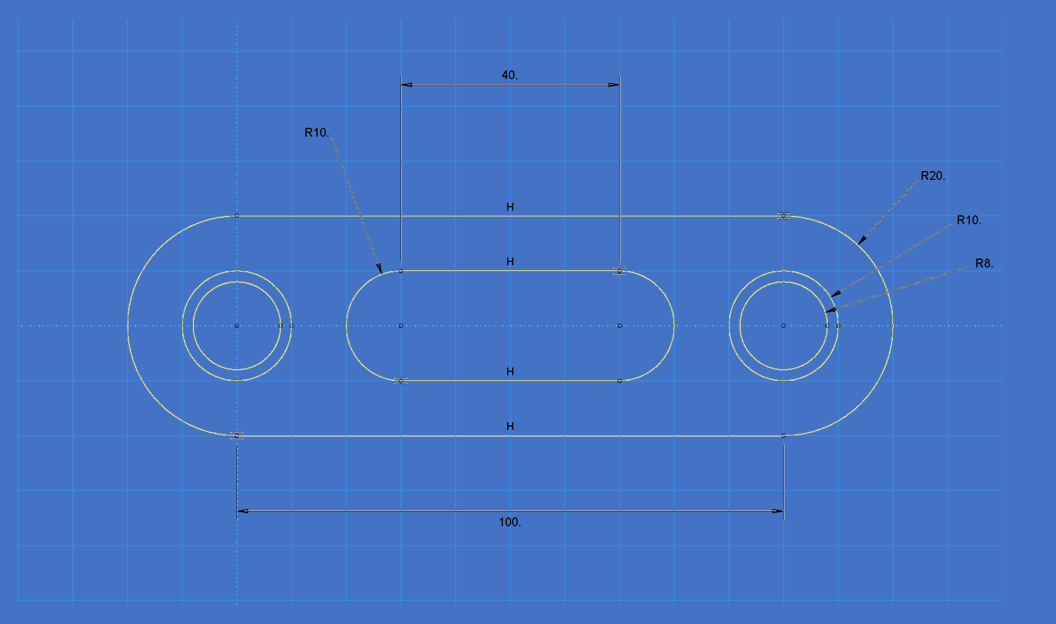
\includegraphics[scale=0.6]{../../images/dimensions_colored.png}
    \caption{Dimensioned torque arm sketch}
    \label{dimensioned_sketch}
\end{figure}

The sole boundary condition applied to the model is on the left hole --- an \textit{encastre} boundary condition constraining all nodal translations and rotations.
Loads are applied as pressures distributed over full surface area of the right hole --- this method of applying the force is not fully physically accurate but does not undermine the analysis of the critical stresses present in the torque arm.
The axial preload is a force with magnitude \(4500\,\unit{\newton}\) while the oscillating component is \(\pm 900\,\unit{\newton}\).
The resulting tractions applied to the right hole are \(11.19\,\unit{\mega\pascal}\) and \(2.24\,\unit{\mega\pascal}\) respectively.
BCs and loads are shown in figure \ref{full_FBD} --- note that the preload and oscillating load are applied in distinct steps.

\begin{figure}[h!]
    \centering
    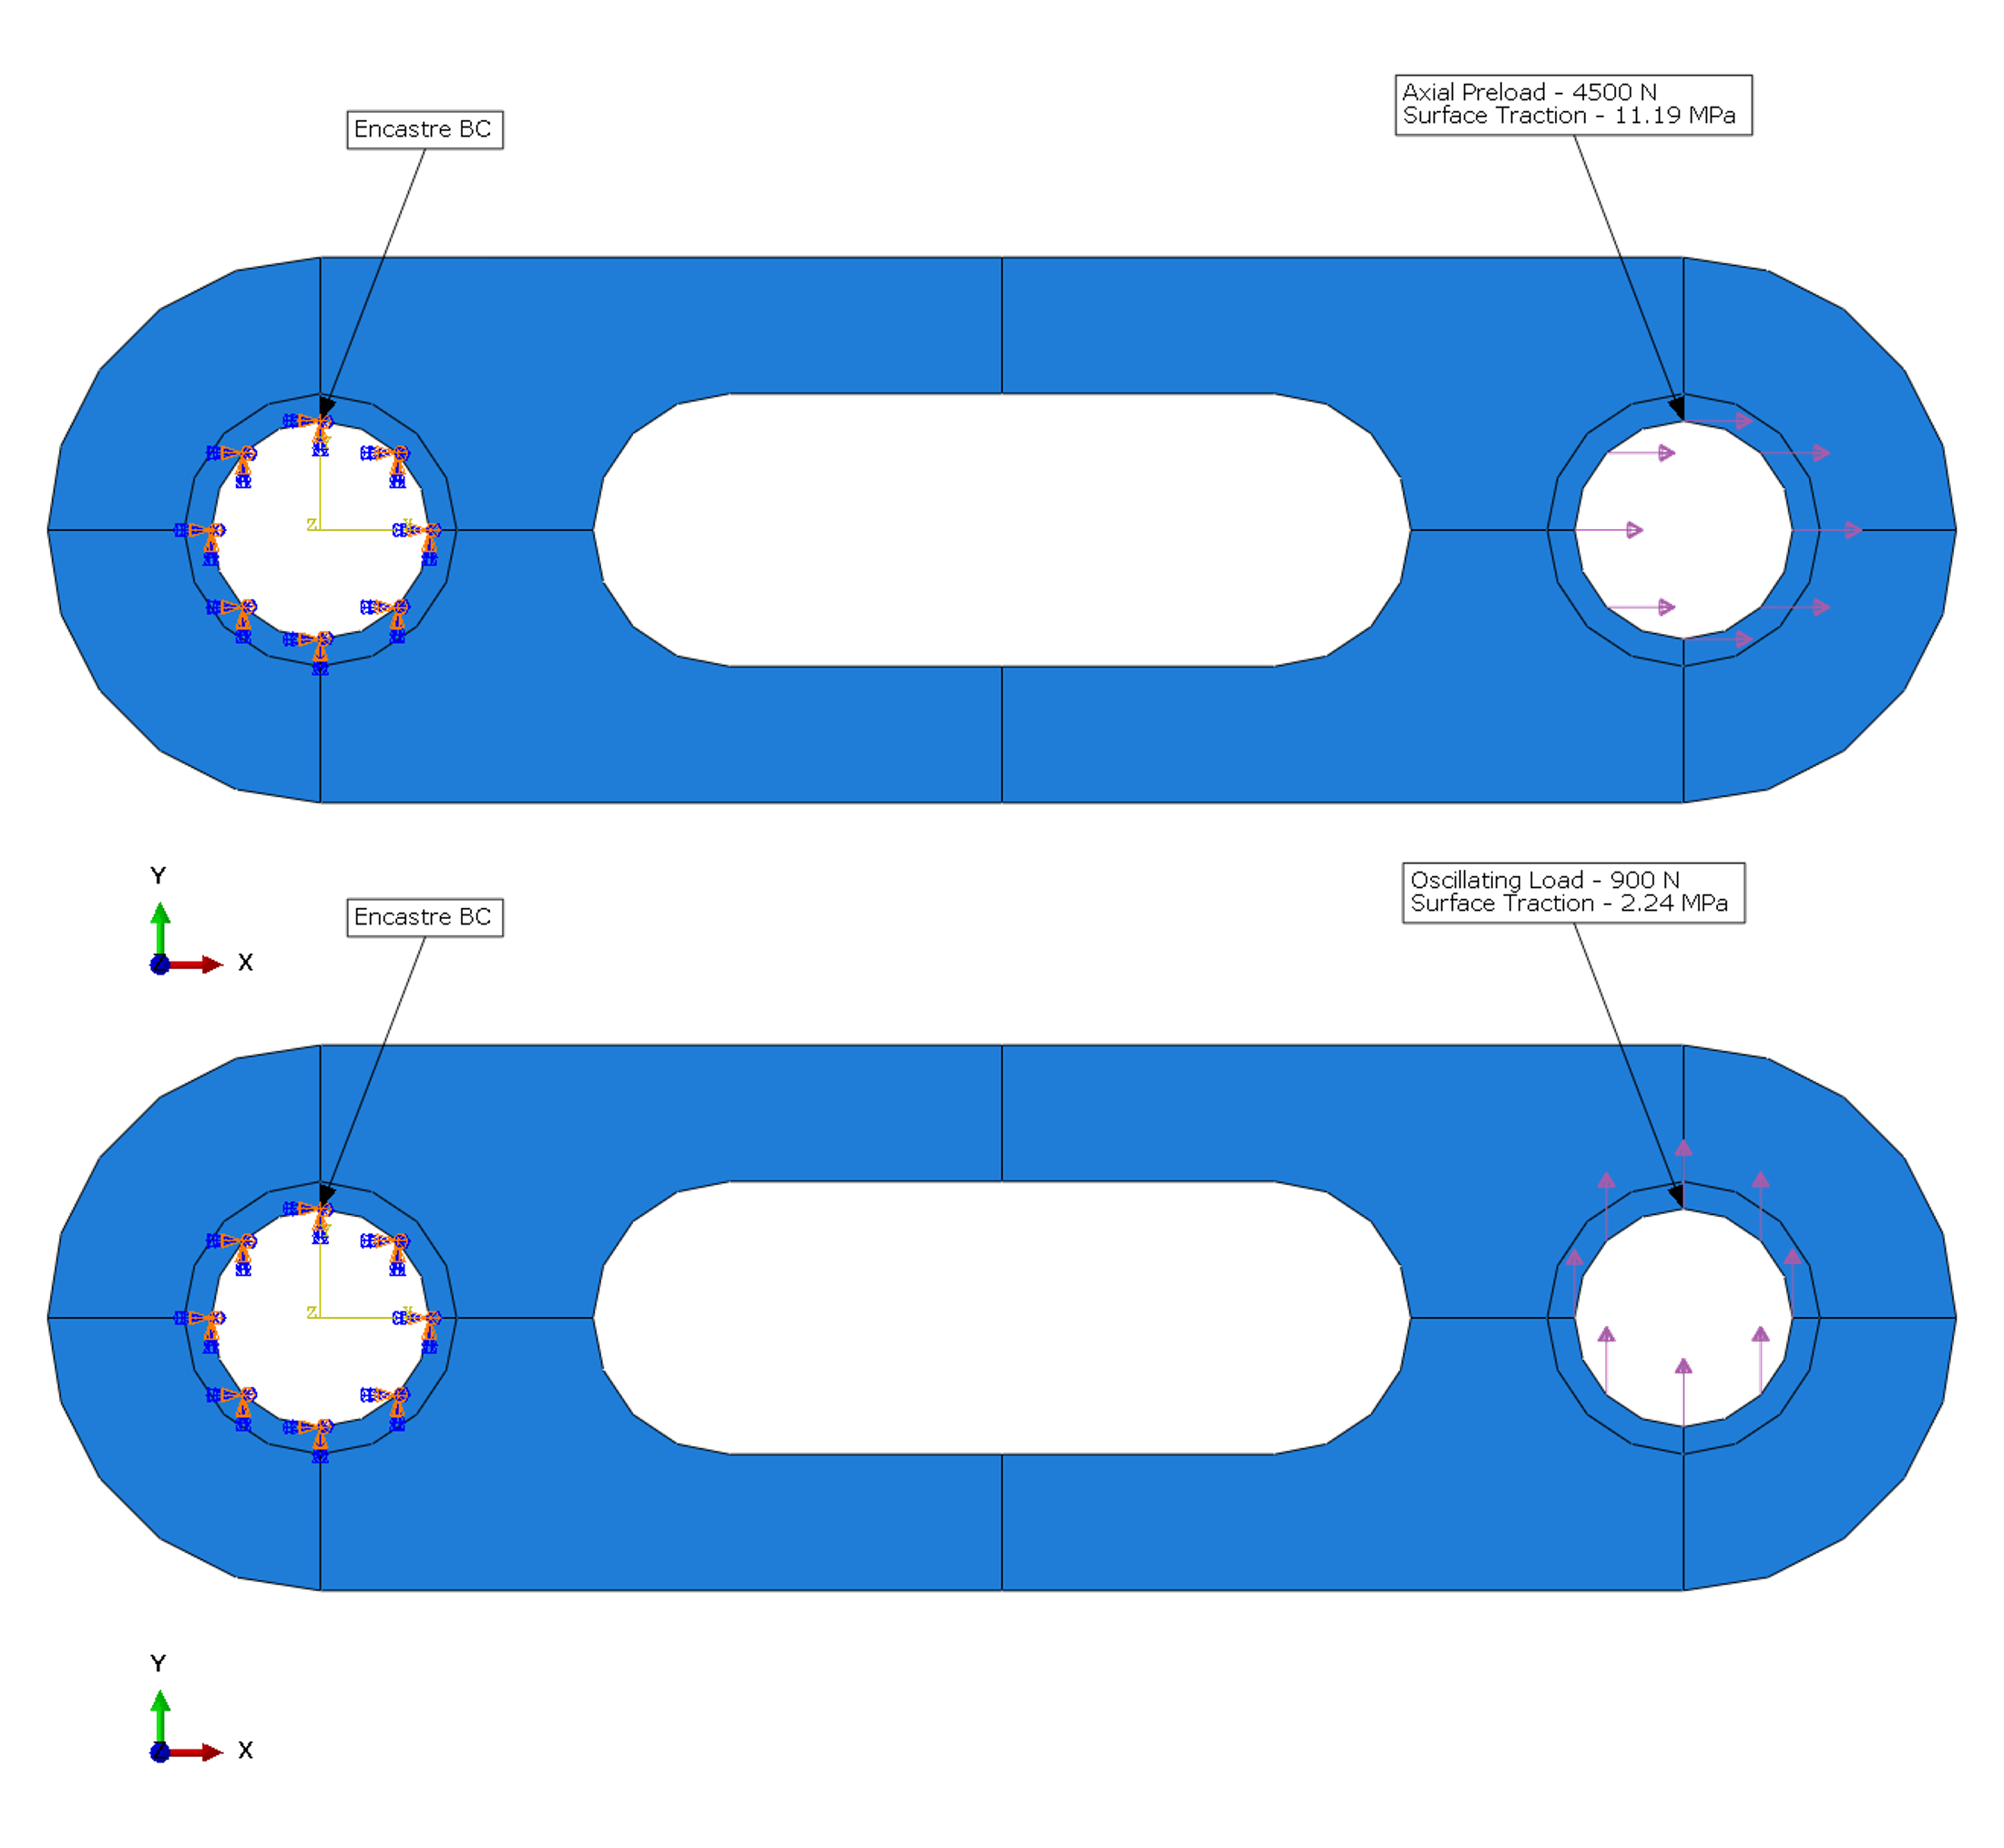
\includegraphics[scale=0.75]{../../images/combined_FBD.png}
    \caption{Preload BC and loads shown on top, oscillating BC and loads shown on bottom.}
    \label{full_FBD}
\end{figure}

The resulting stresses from the two loading cases are analytically combined in post-processing.
The torque arm is modeled as a linear elastic representation of aluminum with Young's Modulus \(E=74.1\,\unit{\giga\pascal}\) and Poisson's Ratio \(\nu=0.33\).
The model is composed of CPS8R elements, 8-node quadratic quadrilateral elements with reduced integration; use of quadratic elements alleviates potential artificial stiffness and more efficiently captures model stresses with a relatively smaller element count than lower-order elements.
The \textit{Abaqus CAE} software mesher automatically generates a mesh on the part instances based on a user-defined model element seed size.
This approach allows for rapid recreation of meshes for convergence studies. 


\end{document}
